\documentclass[aspectratio=169]{../latex_main/tntbeamer}  % you can pass all options of the beamer class, e.g., 'handout' or 'aspectratio=43'
\usepackage{dsfont}
\usepackage{bm}
\usepackage[english]{babel}
\usepackage[T1]{fontenc}
%\usepackage[utf8]{inputenc}
\usepackage{graphicx}
\graphicspath{ {./figures/} }
\usepackage{algorithm}
\usepackage[ruled,vlined,algo2e,linesnumbered]{algorithm2e}
\usepackage{hyperref}
\usepackage{booktabs}
\usepackage{mathtools}

\usepackage{amsmath,amssymb}

\DeclareMathOperator*{\argmax}{arg\,max}
\DeclareMathOperator*{\argmin}{arg\,min}

\usepackage{amsbsy}
\newcommand{\vect}[1]{\bm{#1}}
%\newcommand{\vect}[1]{\boldsymbol{#1}}

\usepackage{pgfplots}
\pgfplotsset{compat=1.16}
\usepackage{tikz}
\usetikzlibrary{trees} 
\usetikzlibrary{shapes.geometric}
\usetikzlibrary{positioning,shapes,shadows,arrows,calc,mindmap}
\usetikzlibrary{positioning,fadings,through}
\usetikzlibrary{decorations.pathreplacing}
\usetikzlibrary{intersections}
\pgfdeclarelayer{background}
\pgfdeclarelayer{foreground}
\pgfsetlayers{background,main,foreground}
\tikzstyle{activity}=[rectangle, draw=black, rounded corners, text centered, text width=8em]
\tikzstyle{data}=[rectangle, draw=black, text centered, text width=8em]
\tikzstyle{myarrow}=[->, thick, draw=black]

% Define the layers to draw the diagram
\pgfdeclarelayer{background}
\pgfdeclarelayer{foreground}
\pgfsetlayers{background,main,foreground}

% Requires XeLaTeX or LuaLaTeX
%\usepackage{unicode-math}

\usepackage{fontspec}
%\setsansfont{Arial}
\setsansfont{RotisSansSerifStd}[ 
Path=../latex_main/fonts/,
Extension = .otf,
UprightFont = *-Regular,  % or *-Light
BoldFont = *-ExtraBold,  % or *-Bold
ItalicFont = *-Italic
]
\setmonofont{Cascadia Mono}[
Scale=0.8
]

\renewcommand{\ttdefault}{Cascadia Mono}

% scale factor adapted; mathrm font added (Benjamin Spitschan @TNT, 2021-06-01)
%\setmathfont[Scale=1.05]{Libertinus Math}
%\setmathrm[Scale=1.05]{Libertinus Math}

% other available math fonts are (not exhaustive)
% Latin Modern Math
% XITS Math
% Libertinus Math
% Asana Math
% Fira Math
% TeX Gyre Pagella Math
% TeX Gyre Bonum Math
% TeX Gyre Schola Math
% TeX Gyre Termes Math

% Literature References
\newcommand{\lit}[2]{\href{#2}{\footnotesize\color{black!60}[#1]}}

%%% Beamer Customization
%----------------------------------------------------------------------
% (Don't) Show sections in frame header. Options: 'sections', 'sections light', empty
\setbeamertemplate{headline}{empty}

% Add header logo for normal frames
\setheaderimage{
	% 
\includegraphics[height=\logoheight]{figures/TNT_darkv4.pdf}
	
\includegraphics[height=\logoheight]{../latex_main/figures/Leibniz-AI-Academy_Logo}
	% 
\includegraphics[height=\logoheight]{figures/logo_tntluh.pdf}
}

% Header logo for title page
\settitleheaderimage{
	% 
\includegraphics[height=\logoheight]{figures/TNT_darkv4.pdf}
	
\includegraphics[height=\logoheight]{../latex_main/figures/Leibniz-AI-Academy_Logo}
	% 
\includegraphics[height=\logoheight]{figures/logo_tntluh.pdf}
}

% Title page: tntdefault 
\setbeamertemplate{title page}[tntdefault]  % or luhstyle
% Add optional title image here
%\addtitlepageimagedefault{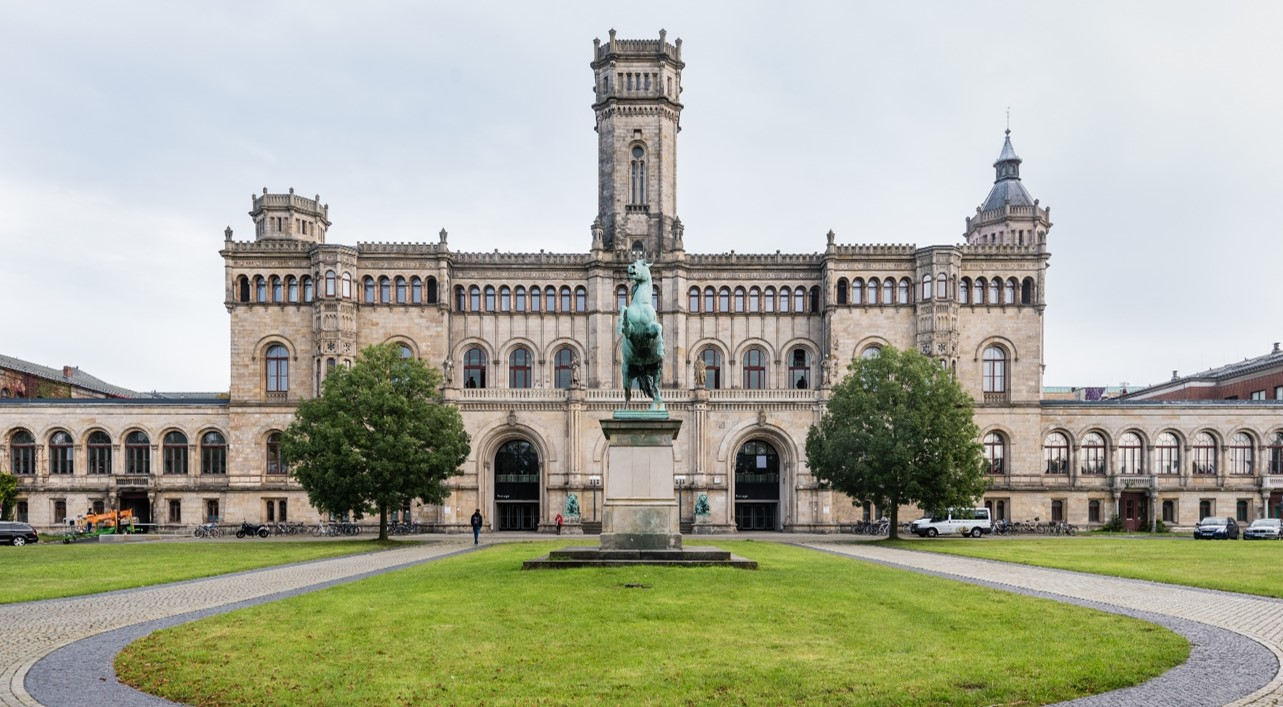
\includegraphics[width=0.65\textwidth]{figures/luh_default_presentation_title_image.jpg}}

% Title page: luhstyle
% \setbeamertemplate{title page}[luhstyle]
% % Add optional title image here
% \addtitlepageimage{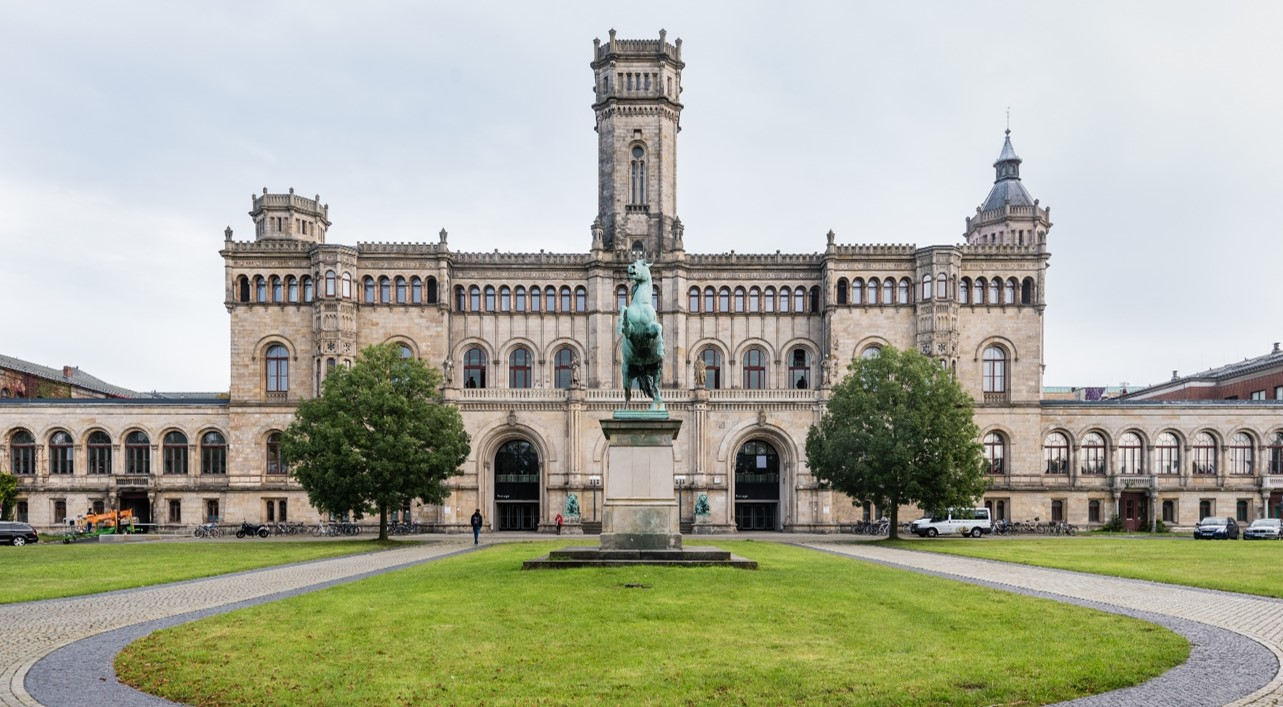
\includegraphics[width=0.75\textwidth]{figures/luh_default_presentation_title_image.jpg}}

\author[Abedjan \& Lindauer]{Ziawasch Abedjan \& \underline{Marius Lindauer}\\[1em]
	%
\includegraphics[height=\logoheight]{../latex_main/figures/luh_logo_rgb_0_80_155.pdf}\qquad
	
\includegraphics[height=\logoheight]{../latex_main/figures/DBIS_Kurzlogo.png}\qquad
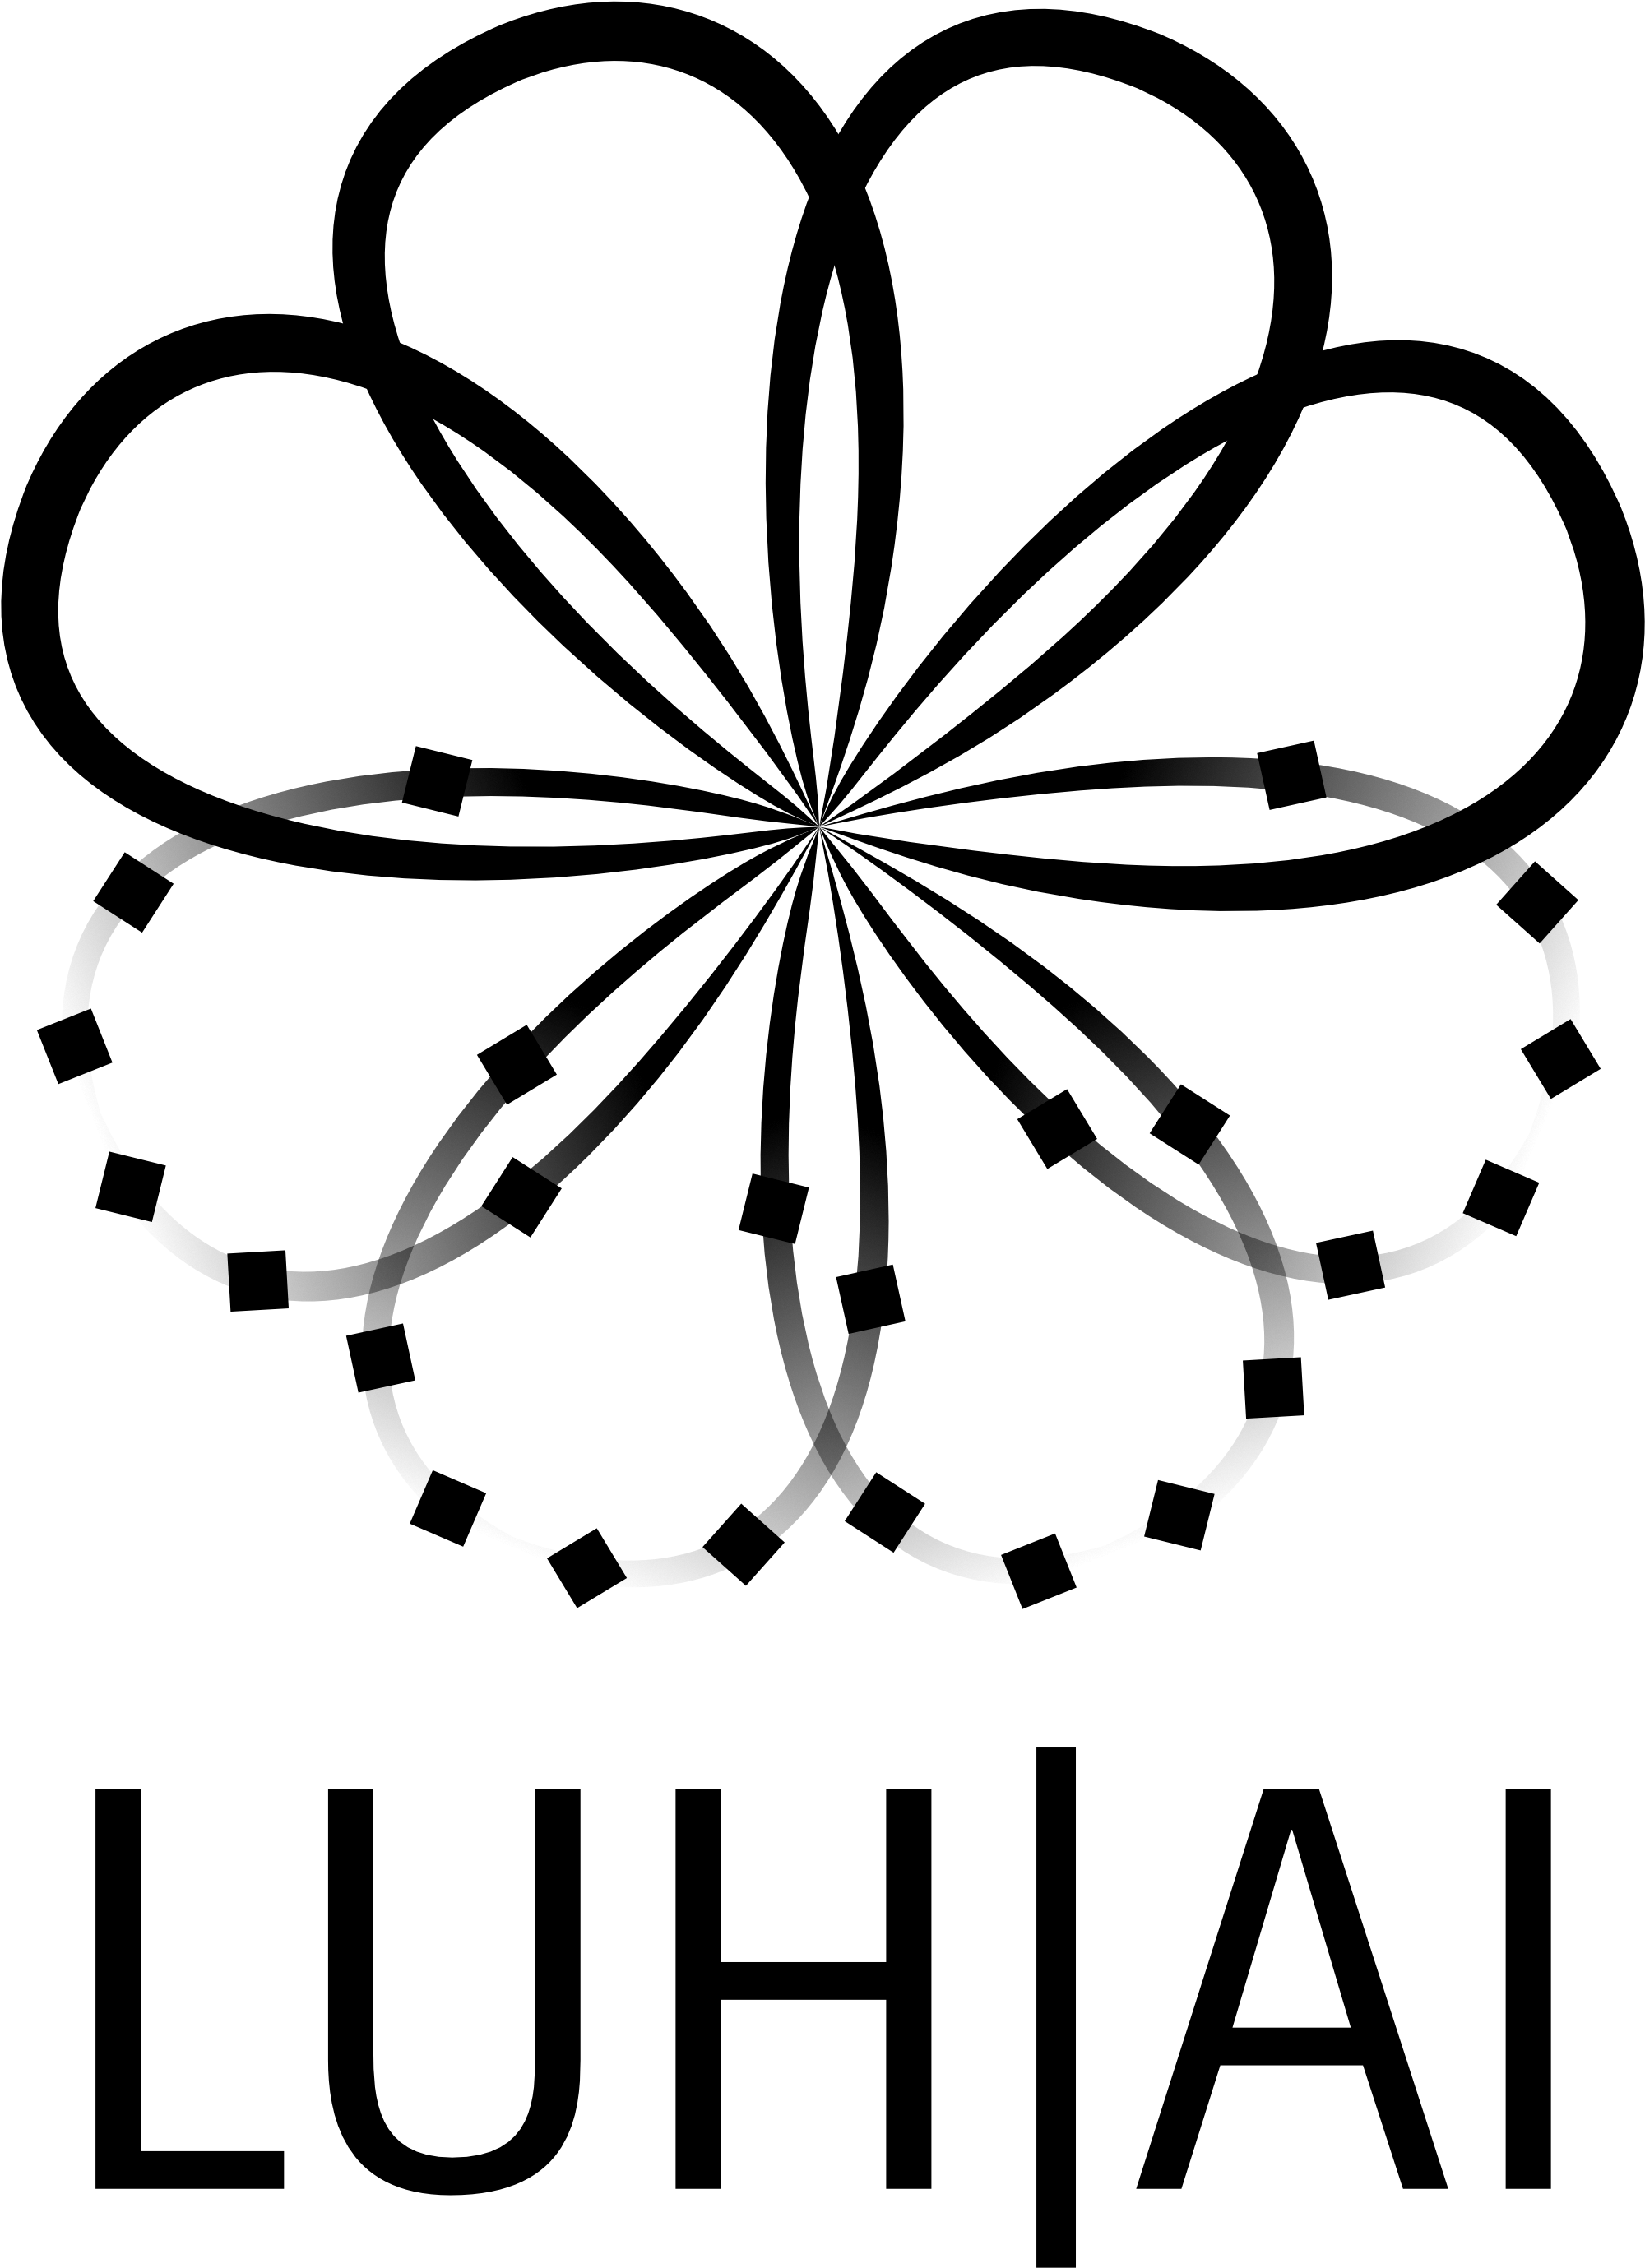
\includegraphics[height=\logoheight]{../latex_main/figures/logo_short_highres_black}\qquad

\includegraphics[height=\logoheight]{../latex_main/figures/Leibniz-AI-Academy_Logo}\qquad
%
\includegraphics[height=\logoheight]{../latex_main/figures/L3S.jpg}	
}
\date{\hspace{0.5em} {
\includegraphics[height=1.5em]{../latex_main/figures/Cc-by-nc-sa_icon.svg.png}}; extension of \href{https://ds100.org/fa21/}{[DS100]}
}


%%% Custom Packages
%----------------------------------------------------------------------
% Create dummy content
\usepackage{blindtext}

% Adds a frame with the current page layout. Just call \layout inside of a frame.
\usepackage{layout}


%%% Macros
%\renewcommand{\vec}[1]{\mathbf{#1}}
% \usepackage{bm}
%\let\vecb\bm

\title[Random Variables]{DS: Data Sampling and Probability}
\subtitle{Random Variables}

\graphicspath{ {./figure/} }
%\institute{}


\begin{document}
	
	\maketitle
	

% Slide 42: Random Variables
\begin{frame}{Random Variable}

    A random variable is a variable that can take numerical values with particular probabilities.\\
    \bigskip
    
    \textbf{Example 1:} \\
    Let $X$ take the value 1 if Roosevelt, 0 if Landon.\\

    \textbf{Example 2:} \\
    Let $Y$ be the number of pips on a roll of a 6-sided die.

    \textbf{Notation:}
    \begin{itemize}
        \item Random variables (RVs) use capital letters, e.g., $X$, $Y$, $Z$.
        \item A particular value taken by an RV is indicated by a lowercase letter, e.g., $x$, $y$, $z$.
        \item The (Probability) Distribution of a discrete RV can be expressed as a table or graphic, e.g., $P(X = x)$.
    \end{itemize}
    

\end{frame}

% Slide 43: Functions of Random Variables
\begin{frame}{Functions of Random Variables}
    
    A function of random variables is also a random variable.
    \bigskip
    
    \textbf{Example 1, cont.:} \\
    Let $S$ be the total number of voters that say “Roosevelt” in a sample of size 10 million.

    \begin{equation}
    S = X_1 + X_2 + \dots + X_{10M}
    \end{equation}


\end{frame}

% Slide 44: Abstracting Random Chance
\begin{frame}{Abstracting Random Chance}

    \textbf{Q:} What do these have in common? \\
    
    \begin{itemize}
        \item Ask a randomly drawn American who they plan to vote for.
        \item The outcome of a coin flip.
        \item The outcome of a COVID test for a randomly selected Californian.
    \end{itemize}
    \pause
    \bigskip

    \textbf{A:} Each has only two outcomes, one of which happens with a particular probability $p$.
\end{frame}

% Slide 45: Bernoulli Distribution
\begin{frame}{Bernoulli Distribution}
    A random variable that takes the value 1 with probability $p$ and 0 otherwise.\\
    
    $X$ is Bernoulli$(p)$ if:
    \begin{equation}
    P(X = 1) = p, \quad P(X = 0) = 1 - p
    \end{equation}

    This is a Probability Mass Function (PMF).\\

    \textbf{Examples:}
    \begin{itemize}
        \item Ask a randomly drawn American who they plan to vote for: Bernoulli$(p = 0.61)$.
        \item The outcome of a coin flip: Bernoulli$(p = 0.5)$.
        \item The outcome of a COVID test for a randomly selected German: Bernoulli$(p = 0.08)$.
    \end{itemize}
\end{frame}

% Slide 46: Abstracting Random Chance
\begin{frame}{Abstracting Random Chance}

    \textbf{Q:} What do these have in common? \\

    \begin{itemize}
        \item Count the number of people that answered “Roosevelt” in a sample of $n = 10$.
        \item The total number of heads in a series of 5 coin flips.
        \item The total number of Germans that will test positive for COVID in a given month.
    \end{itemize}
    \pause
    \bigskip

    \textbf{A:} Each is a sum of Bernoulli random variables.
\end{frame}

% Slide 47: Binomial Distribution
\begin{frame}{Binomial Distribution}
    A random variable that counts the number of "successes" in $n$ independent trials where each succeeds with probability $p$.

    $Y$ is binomial($n,p$) if 
    $$P(Y=y) = \binom{n}{y}p^y(1-p)^{n-y}$$

    Recall: $S = X_1 + X_2 + \ldots + X_{10..}$\\
    S is binomial($n=10, p=0.61$)
\end{frame}

% Slide 48: Abstracting Random Chance
\begin{frame}{Abstracting Random Chance}

    \textbf{Q:} What do these have in common?\\

    \begin{enumerate}
        \item Count the number of people that answered "Roosevelt" in a sample of $n = 10Mio$.
        \item The total number of heads in a series of 5 coin flips.
        \item The total number of Germans that will test positive for COVID in a given month.
    \end{enumerate}


    A random variable that counts the number of “successes” in $n$ independent trials where each succeeds with probability $p$.
    
    \begin{enumerate}
        \item Binomial$(n = 10M, p = 0.61)$ – BUT each $X_i$ is not quite independent with the same $p$.
        \item Binomial$(n = 5, p = 0.5)$ – Good fit!
        \item Binomial$(n = 80M, p = 0.08)$ – Probably not independent (contagious!).
    \end{enumerate}
\end{frame}

% Slide 49: Types of distributions
\begin{frame}{Types of distributions}
    Probability distributions largely fall into two main categories:
    \begin{itemize}
        \item \textbf{Discrete:} 
        \begin{itemize}
            \item The set of possible values that $X$ can take on is either finite or countably infinite.
            \item Values are separated by some fixed amount. 
            \item For instance, $X=1,2,3,4,\ldots$
        \end{itemize} 
        \item \textbf{Continuous:} 
        \begin{itemize}
            \item The set of possible values that $X$ can take on is uncountable.
            \item Typically, $X$ can be any real number in some interval (not just counting numbers).
        \end{itemize} 
    \end{itemize}
    Here, we will focus almost exclusively on discrete distributions, but it’s important to know that continuous distributions exist.
\end{frame}

% Slide 50: Common distributions
\begin{frame}{Common distributions}
    \textbf{Discrete:}
    \begin{itemize}
        \item Bernoulli$(p)$: Takes on the value 1 with probability $p$ and 0 with probability $1 - p$.
        \item Binomial$(n, p)$: Number of 1s in $n$ independent Bernoulli$(p)$ trials. Probabilities are given by the binomial formula.
        \item Uniform on a finite set: Probability of each value is $1 /$ (size of set), e.g., a standard die.
    \end{itemize}

    \textbf{Continuous:}
    \begin{itemize}
        \item Uniform on the unit interval: $U$ could be any real number in the range $[0, 1]$.
        \item Normal distribution $(\mu, \sigma^2)$.
    \end{itemize}
\end{frame}


\end{document}